\documentclass{article}

% Required packages
\usepackage{graphicx}
\usepackage{lipsum} 

% Page configuration
\usepackage[margin=1in]{geometry}

% Title and author
\title{Analysis of AWS Services and characteristics of a distributed application (Performance Monitor)}
\author{}
\date{\today}

\begin{document}

\maketitle

\section{Introduction}

\hspace{1cm} Our application is a distributed system consisting of various components that are hosted on the AWS cloud platform. This scientific report aims to analyze these AWS services used in our application architecture and evaluate their characteristics. 

\begin{figure}[htbp]
    \centering
    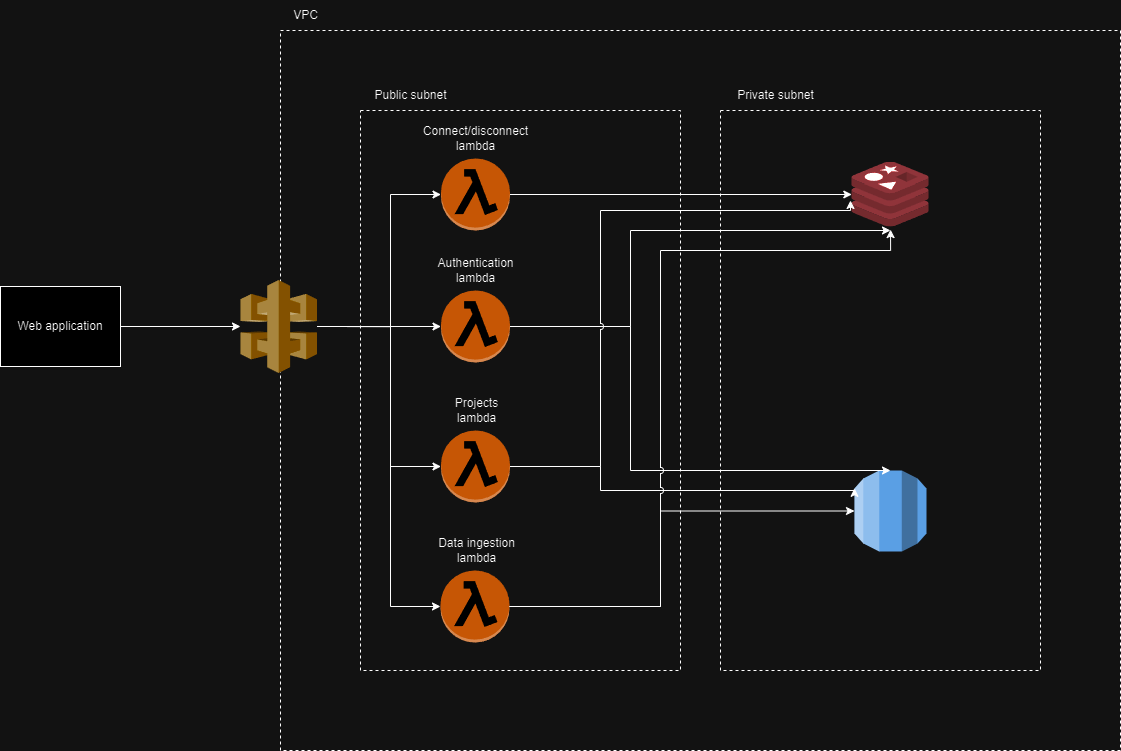
\includegraphics[width=0.9\textwidth]{pcd2.drawio (1).png}
    \caption{Arhitecture Diagram}
    \label{fig:diagrama}
\end{figure}

\section{Arhitecture}

\hspace{1cm} We designed a distributed system with a client-server architecture that provides scalability, modularity, and effective resource management. The two main elements are:

\subsection{Client component}

\hspace{1cm}The user interface, which is in charge of facilitating direct communication with end users, is represented by the client component. The React web application acts as a representation of this in our scenario. The client program controls all aspects of record processing and result display, while the server processes requests from the client and returns results.

\subsection{Server component}

\hspace{1cm}The backend of the application, which handles business logic, data processing, and storage, is represented by the server component. In this case, AWS services like Redis, Amazon RDS, API Gateway, and AWS Lambda represent this component. The client sends requests to the server, which uses business logic to process them and then sends the results back to the client.


\begin{itemize}
    \item \textbf{API Gateway with WebSockets}: Our API endpoints are managed by Amazon API Gateway, which also offers support for WebSocket communication. API Gateway WebSocket APIs are bidirectional.Services can send messages to clients on their own, and clients can send messages to services. Because of this bidirectional behavior, that allows services to push data to clients without explicitly requesting it, clients and the backend infrastructure can have richer interactions. 
    \item \textbf{AWS Lambda Functions}: According to the AWS documentation Lambda runs the code on a high-availability compute infrastructure and performs all of the administration of the compute resources, including server and operating system maintenance, capacity provisioning and automatic scaling, and logging. We use four AWS Lambda functions-Connect/Disconnect/Authentication/Data Ingestion- to handle various aspects of our application logic. These serverless functions provide scalable and economical processing by executing code in response to being triggered by events.
    \item \textbf{Redis}: Redis is a source available software that serves as an in-memory data store to speed up our application by caching frequently accessed information. It helps to lower latency for some processes by providing quick read and write operations.
    \item \textbf{Amazon RDS with PostgreSQL}: We use the relational database management system PostgreSQL with Amazon RDS for durable data storage. Our data is protected by this managed database service, which provides scalability, dependability, and automated backups for disaster recovery.
    \item \textbf{Virtual Private Cloud (VPC)}: In order to isolate our resources and offer better security, every component of our application is deployed inside a Virtual Private Cloud (VPC). This lets us specify the public and private subnets, routing tables, and IP ranges that compose our network environment.
    
\end{itemize}

\section{Analysis of System Characteristics}


\subsection{Performance}

\hspace{1cm} AWS Lambda's serverless architecture makes sure that processing power is used effectively, while Redis caching decreases latency when retrieving information. With elastic scaling features available through AWS services, the architecture is built to be scalable. While AWS Lambda automatically adjusts its scalability to meet demand changes, Amazon RDS enables us to adjust our database resources either vertically or horizontally according with workload demands. It might, however, experience performance issues when dealing with a large number of simultaneous requests, much like Twitter at periods of high usage.

\subsection{Latency}

\hspace{1cm} Our application responds more quickly because real-time, low-latency communication is made possible by using WebSocket communication over API Gateway. Furthermore, the distributed architecture of AWS services guarantees low-latency data processing and access.

\subsection{Reliability}

\hspace{1cm}Because of their automatic failover methods, frequent backups, and built-in redundancy, AWS services are highly reliable. While AWS Lambda offers fault tolerance with automatic scaling and replication across several availability zones, Amazon RDS guarantees data durability with automated backups and multi-AZ options for deployment.


\subsection{Transparency}

\hspace{1cm}AWS services offer powerfull tools for monitoring and logging to guarantee the transparency of our system. We use AWS CloudWatch to look at our application's functioning staten and efficiency in real time. We also log all API calls and actions executed within our AWS environment using AWS CloudTrail. This service gives us visibility into user activity and system modifications. We can promptly detect and resolve problems thanks to these transparency features, which guarantees the dependability and availability of our program.

\section{Conclusions}

\hspace{1cm}In conclusion, despite the fact that our application is still in its early stages of development, we have built a strong basis for creating a reliable and effective distributed application. Our architectural approach makes use of AWS's scalability, stability, and security characteristics. Future development paths can include optimizing security by encrypting sensitive data using AWS Key Management Service (KMS) and performance by using AWS Auto Scaling to automatically modify computing power to manage variable amounts of demand.

\end{document}
